\documentclass[../main.tex]{subfiles}
\usepackage{fancyhdr}
\graphicspath{{../images/}}

\begin{document}
\pagestyle{fancy}
\lhead{Physics 472: Li Yang}
\chead{Homework 1}
\rhead{Junseo Shin}

\renewcommand\thefigure{\arabic{figure}} 
\paragraph*{1.} For the HCP structure ABAB\dots the atoms in the B layer are equidistant from the atoms
in the lower basal plane. The distance between an atom in the A layer and the atom in the B layer
is equivalent to the distance between the atoms in the basal plane $a$. Also the height of the B
layer is $c/2$. We can draw a right triangle with the hypothenuse being the distance between the atoms $a$ and
two sides of length $c/2$ and $x$ as shown in Figure \ref{fig:hw1_1}.

\begin{figure}[ht]
    \centering
    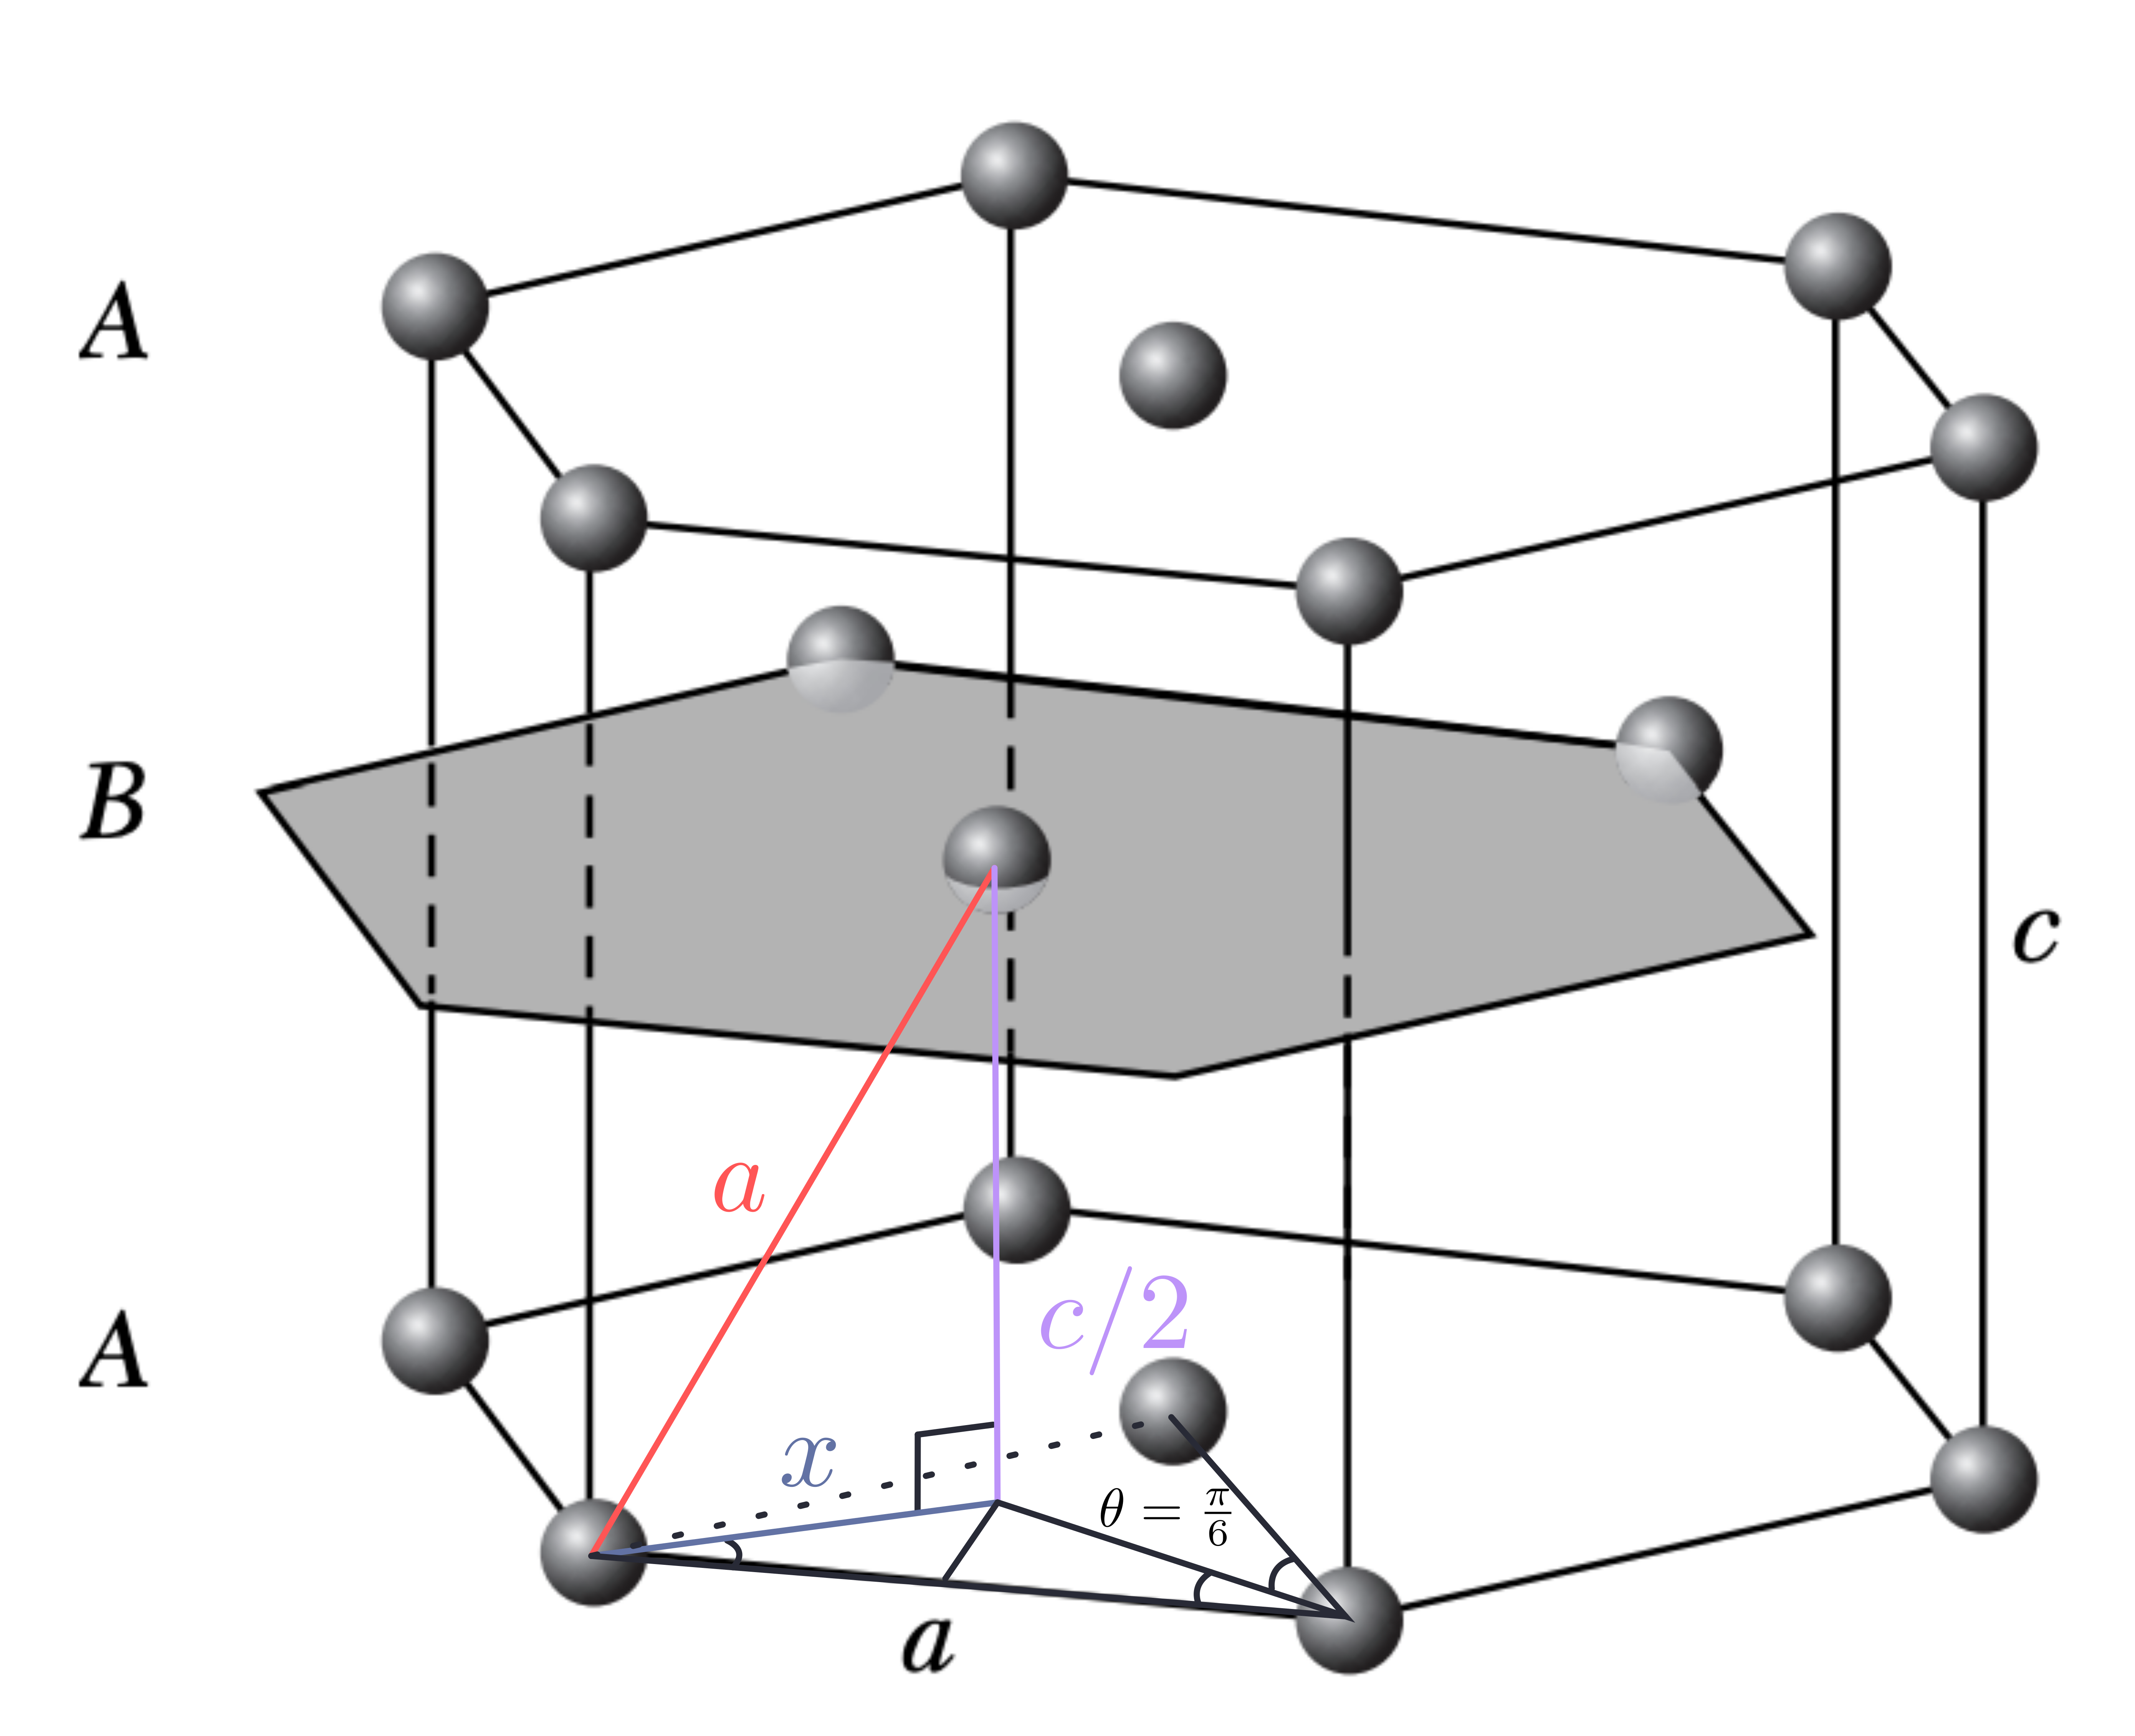
\includegraphics[width=0.4\textwidth]{hw1_1.png}
    \caption{HCP structure (From Kittel)}
    \label{fig:hw1_1}
\end{figure}
To find $x$ we can project the B atom onto the basal plane and
use trig to find that
\begin{align*}
    x \cos{\frac{\pi}{6}} &= \frac{a}{2} \to x = \frac{a}{\sqrt{3}}
\end{align*}
So using the Pythagorean theorem we can find the distance between the atoms in the A and B layers
\begin{align*}
    a^2 &= \qt(\frac{c}{2})^2 + x^2 \\
    a^2 &= \frac{c^2}{4} + \qt(\frac{a}{\sqrt{3}})^2 \\
    \frac{2}{3} a^2 &= \frac{c^2}{4} \\
    \frac{c}{a} &= \sqrt{\frac{8}{3}} \approx 1.633
\end{align*}

\paragraph*{2.} (a) Given
\begin{align*}
    \vb{a}_1 = (\sqrt{3}a/2) \vu{x} + (a/2) \vu{y}; \qquad 
    \vb{a}_2 = -(\sqrt{3}a/2) \vu{x} + (a/2) \vu{y}; \qquad
    \vb{a}_3 = c \vu{z}
\end{align*}
the volume of the primitive cell is equivalent to the volume of the parallelepiped:
\begin{align*}
    V_c &= \vb{a}_1 \cdot (\vb{a}_2 \cross \vb{a}_3) \\
    &= \vb{a}_1 \cdot \det\begin{vmatrix}
        \vu{x} & \vu{y} & \vu{z} \\
        -\sqrt{3}a/2 & a/2 & 0 \\
        0 & 0 & c
    \end{vmatrix} \\
    &= \qt(\frac{\sqrt{3}a}{2} \vu x + \frac{a}{2} \vu{y}) \cdot 
    \qt(\frac{ac}{2} \vu{x} + \frac{\sqrt{3}ac}{2} \vu{y}) \\
    &= \frac{\sqrt{3}a^2c}{4} + \frac{\sqrt{3}a^2c}{4} \\
    &= \frac{\sqrt{3}a^2c}{2}
\end{align*}
(b) The first reciprocal lattice vector is
\begin{align*}
    \vb{b}_1 &= 2\pi \frac{\vb{a}_2 \cross \vb{a}_3}{V_c} \\
    &= 2\pi \frac{\qt(\frac{ac}{2} \vu{x} + \frac{\sqrt{3} ac}{2} \vu{y})}{\frac{\sqrt{3}a^2c}{2}} \\
    &= 2\pi \frac{\vu{x} +  \sqrt{3} \vu{y}}{\sqrt{3}a} \\
    &= \frac{2\pi}{a} \qt(\frac{1}{\sqrt{3}} \vu{x} + \vu{y})
\end{align*}
The other reciprocal lattice vectors can be found similarly:
\begin{align*}
    \vb{a}_3 \cross \vb{a}_1 &= \det\begin{vmatrix}
        \vu{x} & \vu{y} & \vu{z} \\
        0 & 0 & c \\
        \sqrt{3}a/2 & a/2 & 0
    \end{vmatrix} = -\frac{ac}{2} \vu{x} + \frac{\sqrt{3}ac}{2} \vu{y}
\end{align*}
so
\begin{align*}
    \vb{b}_2 &= 2\pi \frac{\vb{a}_3 \cross \vb{a}_1}{V_c}
    = \frac{2\pi}{a} \qt(-\frac{1}{\sqrt{3}} \vu{x} + \vu{y})
\end{align*}
and 
\begin{align*}
    \vb{a}_1 \cross \vb{a}_2 = \det\begin{vmatrix}
        \vu{x} & \vu{y} & \vu{z} \\
        \sqrt{3}a/2 & a/2 & 0 \\
        -\sqrt{3}a/2 & a/2 & 0
    \end{vmatrix} = (\sqrt{3}a^2/4 + \sqrt{3}a^2/4) \vu{z} = \frac{\sqrt{3}a^2}{2} \vu{z}
\end{align*}
so
\begin{align*}
    \vb{b}_3 &= 2\pi \frac{\vb{a}_1 \cross \vb{a}_2}{V_c} = \frac{2\pi}{c} \vu{z}
\end{align*}

(c) A sketch of the 2D Brillouin zone is a hexagon as shown in Figure \ref{fig:hw1_2}.
\begin{figure}[ht]
    \centering
    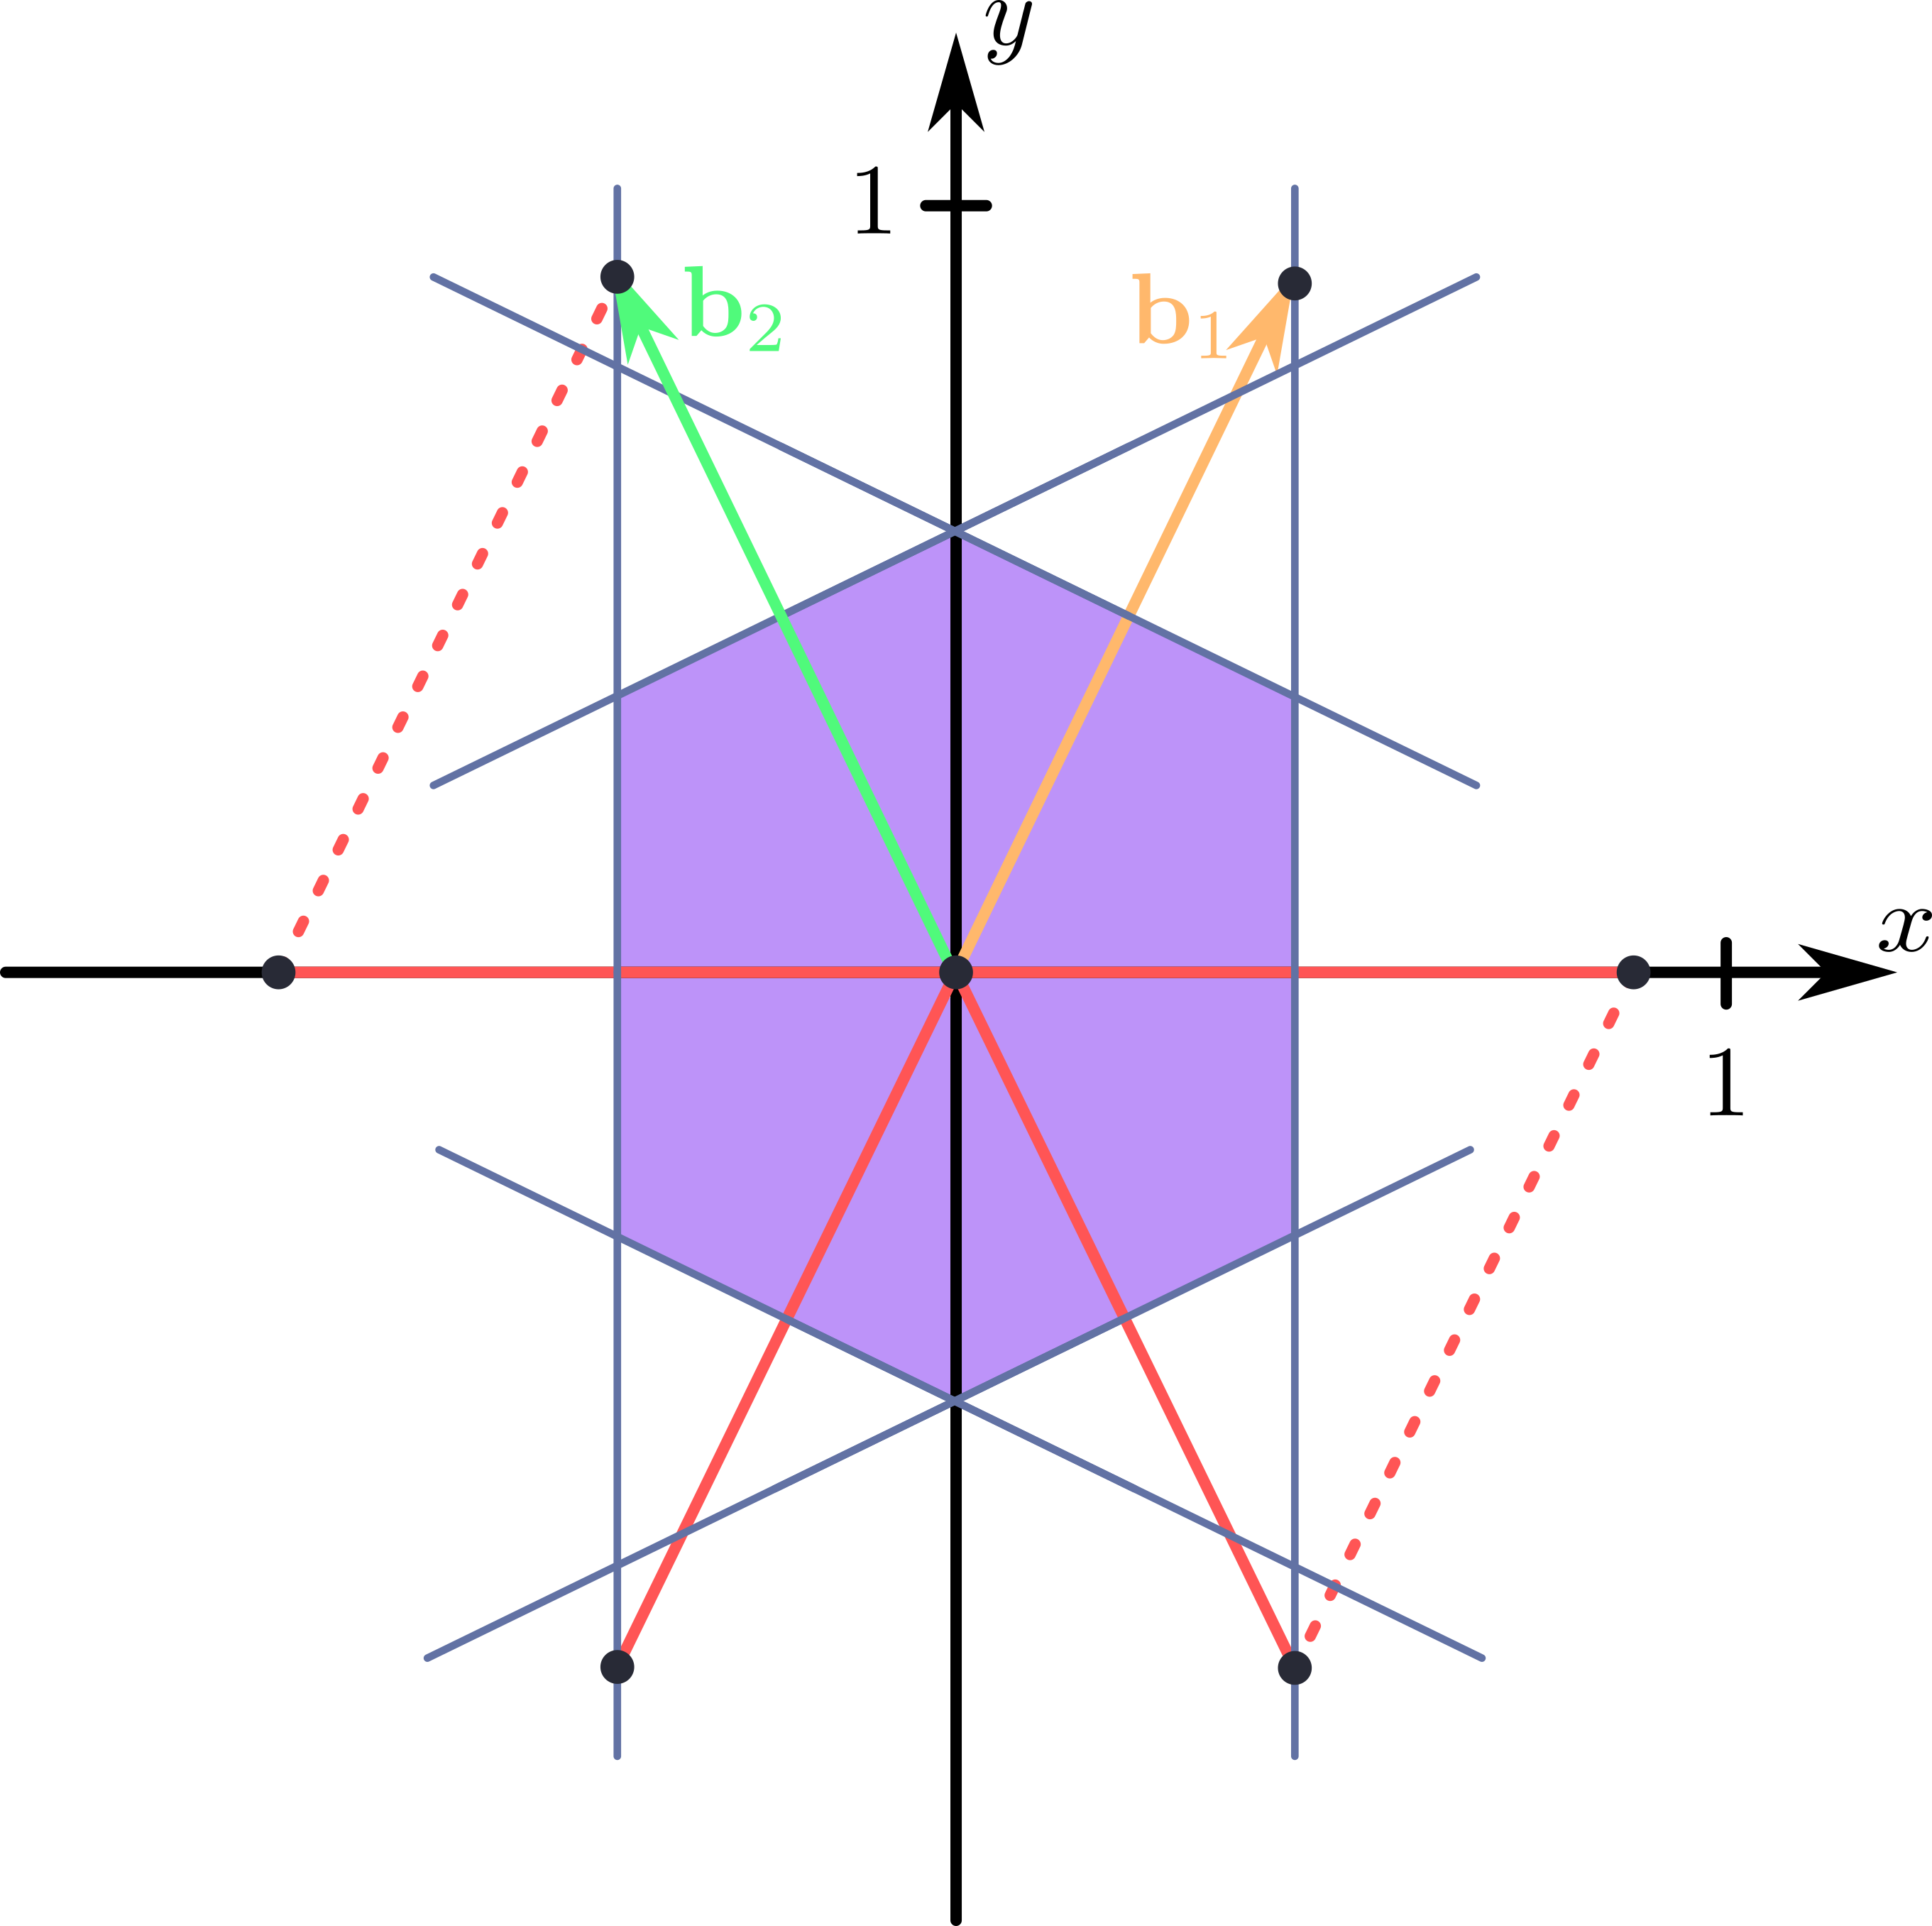
\includegraphics[width=0.4\textwidth]{hw1_2.png}
    \caption{2D Brillouin zone on $xy$ plane}
    \label{fig:hw1_2}
\end{figure}

\paragraph*{3.} (a) The total potential energy is 
\begin{align*}
    U(R) &= N \qt(\frac{A}{R^n} - \frac{\alpha q^2}{R}) \\
\end{align*}
where the Madelung constant for a 1D chain of ions is $\alpha = 2 \ln{2}$, and we replace the 
usual repulsive potential $\lambda \exp(-R/p)$ with $A/R^n$. Taking the derivative with respect to
$R$ an finding the equilibrium seperation at a critical point:
\begin{align*}
    \dv{U}{R} &= N \qt(-\frac{nA}{R^{n+1}} + \frac{\alpha q^2}{R^2}) = 0 \\ 
    \frac{NA}{R^{N+1}} &= \frac{\alpha q^2}{R^2} \\
    \frac{R^{n+1}}{R^2} &= \frac{nA}{\alpha q^2} \\
    R_o^{n-1} &= \frac{nA}{\alpha q^2} \\
    A &= \frac{\alpha q^2 R_o^{n-1}}{n}
\end{align*}
substituting back into the potential energy:
\begin{align*}
    U(R_o) &= N \qt(\frac{\alpha q^2 R_o^{n-1}}{nR_o^n} - \frac{\alpha q^2}{R_o}) \\
    &= N \qt(\frac{\alpha q^2}{nR_o} - \frac{\alpha q^2}{R_o}) \\
    &= \frac{N\alpha q^2}{R_o} \qt(\frac{1}{n} - 1) \\
    U(R_o) &= -\frac{2N q^2\ln{2}}{R_o} \qt(1 - \frac{1}{n})
\end{align*}
(b) Approximating the potential around $x$ using Taylor expansion
$f(x + h) = f(x) + f'(x) h + \frac{1}{2} f''(x) h^2$:
\newcommand{\rapr}{(R_o\delta)}
\begin{align*}
    U(R_o(1 - \delta)) &= U(R_o + (- R_o\delta))  \\
    &= U(R_o) - [U'(R_o)] \rapr + \frac{1}{2}[U''(R_o)] \rapr^2 + \dots \\
\end{align*}
and since $\dv{U}{R} = 0$ at $R_o$, the second term is zero. And the second order derivative gives
\begin{align*}
    \dv[2]{U}{R} &= N \qt(\frac{n(n+1)A}{R^{n+2}} - \frac{2\alpha q^2}{R^3})\eval_{R=R_o} \\
    \qusing R_o^{n-1} &= \frac{nA}{\alpha q^2} \\
    &= N \qt(\frac{n(n+1)A}{\frac{nA}{\alpha q^2} R_o^3} - \frac{2\alpha q^2}{R_o^3}) \\
    &= N \qt(\frac{(n+1)\alpha q^2}{R_o^3} - \frac{2\alpha q^2}{R_o^3}) \\
    &= \frac{N\alpha q^2}{R_o^3} ((n+1) - 2) \\
    \dv[2]{U}{R} &= \frac{N\alpha q^2}{R_o^3} (n - 1)
\end{align*}
so potential is approximately
\begin{align*}
    U(R_o(1 - \delta)) &\approx U(R_o) + \frac{1}{2} \frac{N\alpha q^2}{R_o^3} (n - 1) \rapr^2
\end{align*}
so the leading coefficient is (ignoring the $\frac{1}{2}\delta^2$ part)
\begin{align*}
    C = \frac{N\alpha q^2}{R_o^3} (n - 1) R_o^2
\end{align*}
To cancel the $N$ we can use that fact that compressing to the unit length makes the seperation
between ions $2NR_o = 1$, so $N = 1/(2R_o)$, so
\begin{align*}
    C &= \frac{1}{2R_o} \frac{\alpha q^2}{R_o^3} (n - 1) R_o^2 = \frac{\alpha q^2}{2R_o^2} (n - 1)
\end{align*}
and using the Madelung constant $\alpha = 2\ln{2}$, the leading term is finally
\begin{align*}
    C = \frac{(n - 1)q^2 \ln{2}}{R_o^2} 
\end{align*}
so the work done is
\begin{align*}
    W &= \Delta U = U(\rapr) - U(R_o) \\
    &\approx U(R_o) + \frac{1}{2} C \delta^2 - U(R_o) \\
    W &\approx \frac{1}{2} C^2 \delta^2
\end{align*}
where the leading term is indead in the order of $\frac{1}{2} C \delta^2$. 
\end{document}